\chapter{Analysis and Results}
\label{cap:AnalysisandResults1}

This chapter presents the analysis and results of standby traffic and event captures. First the analysis of standby traffic is analysed to identify traffic irrelevant to the events objectives triggered. This is followed by a section for each event including analysis of overall event characteristics, protocol detection and packet sequences, which results in a signature. WAN traffic is compared with the corresponding WLAN traffic to identify if these signatures are applicable in both transmissions domains. 

\section{Standby Traffic}
This section presents the analysis of the captured standby traffic to identify traffic pattern  or protocols to create a base filter to excluding them for further event analysis. First an analysis of the relevance of different identified protocols is conducted. All occurring traffic patterns within the standby event can be found in the event captures as well, but are irrelevant for the actual event triggering.

The standby event capturing was conducted from 8th of January to 22th of January 2023 in Oslo test environment. During this time period there was no physical or application interacting with the Irobot Roomba, all traffic captured was then generated by the Irobot Roomba or connected Irobot cloud service. This traffic is therefore not created by any human interaction and not exposing any private information. Beforehand the Irobot Roomba had been installed and operated for 1 month, ensuring that it was in a operation and not installation state. Smart home map, room dividers and customized  cleaning jobs were configured. 

Wireshark protocol hierarchy analysis tool was used to display protocol statistics identified by Wireshark, Table \ref{tab:ProtocolStatistics} presents the protocols and distribution of them. Approximately 50\% of the captured traffic was identified as UDP traffic this is mainly DNS by also some NTP and DHCP traffic. 26.2\% was TCP where the majority of the captured traffic is TLS which is used by the Irobot Roomba to ensure end-to-end encryption of the cloud communication. The last protocol identified was ARP representing 24,6\% of the standby traffic. 


\begin{table}[H]
\centering
\caption{Protocol hierarchy and statistics in standby capture }
\label{tab:ProtocolStatistics}
\begin{tabular}{|l|l|l|l|}
\hline
\multicolumn{1}{|c|}{\textbf{Transport protocol}} & \textbf{Percentage}     & \textbf{Service protocol} & \textbf{Percentage} \\ \hline
\multirow{3}*{UDP}                              & \multirow{3}*{49,2} & DHCP    & 0,1            \\ \cline{3-4} 
                                                  &                         & DNS                       & 48,6                \\ \cline{3-4} 
                                                  &                         & NTP                       & 0,4                 \\ \hline
TCP                                               & 26,2                    & NA                        & NA                  \\ \hline
ARP                                               & 24,6                    & NA                        & NA                  \\ \hline
\end{tabular}
\end{table}

The network architecture in Oslo and Drammen creates a single boradcast domain between the AP, capturing platform and the ISP router, as the capturing platform only collects traffic from the LAN it is not generating any traffic. As devices only use physical layer MAC addresses to communicate on the LAN they need ARP to create a IP to MAC forwarding table. ARP traffic is therefore broadcasted between these two devices requesting updates on IP tp MAC information. The captured ARP traffic is not generated by the vacuum cleaner in another broadcast domain and is added as a part of the base filter with the logical expression \textit{!arp}.

The ISP modem is by default configured as the local DHCP server allocating, reserving and leasing IP addresses to devices connection to the LAN. It ease the detection of the simulated WAN traffic a DHCP reservation was configured on the ISP routers for the AP's LAN MAC address in Oslo and Drammen. This kept the simulated WAN address from changing IP during capturing and potentially lose traffic. DHCP traffic still was needed to be exchanged between the AP and the ISP modems requesting and verifying that the reserved DHCP lease still was active during capturing. DHCP traffic in the LAN capture is therefore only generated by the AP and the ISP modem and was added to the base filter with the logical expression \textit{!dhcp}.

The most dominant protocol in the standby capture was DNS with 49.2\% of the packets, 98.3\% of all these DNS packets was requests and responses for the DNS A record of \textit{a.root-servers.net}, this traffic flow is shown through Wireshark in Figure \ref{fig:dns_a-root}. This is one of the DNS top level domain servers in the DNS hierarchy and will only point to top level domain server such as .com, .org and .no. By analyzing the management console of the AP it was observed that the AP requested the DNS record for \textit{a.root-servers.net} to determine if had Internet connectivity or not. A successful response will indicate Internet connectivity. These DNS packets are therefore irrelevant in the analysis of Irobot Roomba traffic and are specifically excluded in a Wireshark filter for further DNS analysis with the following filter  \textit{(dns) \&\& !(frame.len ==78 or frame.len ==94)} to the Wireshark filter. Frame lengths of 78 and 94 bytes are used to identify the DNS request and response in Figure  \ref{fig:dns_a-root}

\begin{figure}[H]
    \centering
    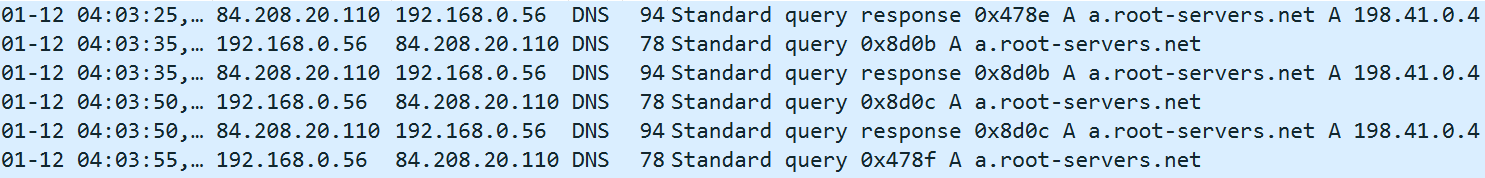
\includegraphics[width=\textwidth]{figures/DNS_a-root.png}
    \caption{Reoccurring DNS traffic towards a.root-server.net}
    \label{fig:dns_a-root}
\end{figure}

174 DNS packets was left after excluding removing the top level domain requests from the other DNS traffic. In the remaining DNS traffic it is observed several DNS requests and responses generated by the AP towards the TP-Link cloud services, these FQDNs are listed below, and shown in Figure \ref{fig:tp-link_fqdn}. 

\begin{itemize}
    \item n-devs-gw.tplinkcloud.com
    \item n-deventry-gw.tplinkcloud.com
\end{itemize}

\begin{figure}[H]
    \centering
    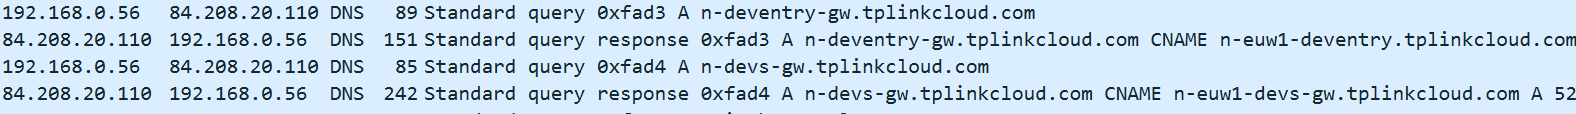
\includegraphics[width=\textwidth]{figures/DNS-tp-link.png}
    \caption{DNS traffic generated by the AP towards TP-LInk could services}
    \label{fig:tp-link_fqdn}
\end{figure}

These DNS packets are excluded and only four different FQDN requests generated by the Irobot Roomba is displayed. Three of the FQDN are towards \textit{.irobot} domain and the last one is a part of \textit{amazoneaws}. Amazone AWS is a large provider of cloud services and bought Irobot cooperation in 2022 \cite{irobot2023_amazone} and is therefore using Amazone AWS for their cloud services. These FQDNs are listed below. 

\begin{itemize}
    \item 0.irobot.pool.ntp.org
    \item disc-prod.iot.irobotapi.com
    \item unauth1.prod.iot.irobotapi.com
    \item a2uowfjvhio0fa.iot.us-east-1.amazonaws.com
\end{itemize}

All DNS traffic generated by the Irobot Roomba are occurring regularly throughout the entire standby traffic time period, this is presented in Figure \ref{fig:dns_irobot_graph}. Irobot's public NTP server \textit{0.irobot.pool.ntp.org} is requested each 12th hour,  in the standby traffic this is at 03:36 and 15:36. This is used to synchronize the local clock on the Irobot Roomba to a global time zone, allowing all actions or smart features using time to operate correct. \textit{disc-prod.iot.irobotapi.com}, \textit{unauth1.prod.iot.irobotapi.com} and \textit{a2uowfjvhio0fa.iot.us-east-1.amazonaws.com} are all requested once a day at the same time. The function of these requests are not identified, but when trying to access the FQDNs through a Google Chrome it prompts \textit{"Missing Authentication Token"}, based on the naming convention of the FQDNs it is easy to believe that they are used for re-authentication of the Irobot Roomba. 

\begin{figure}[H]
    \centering
    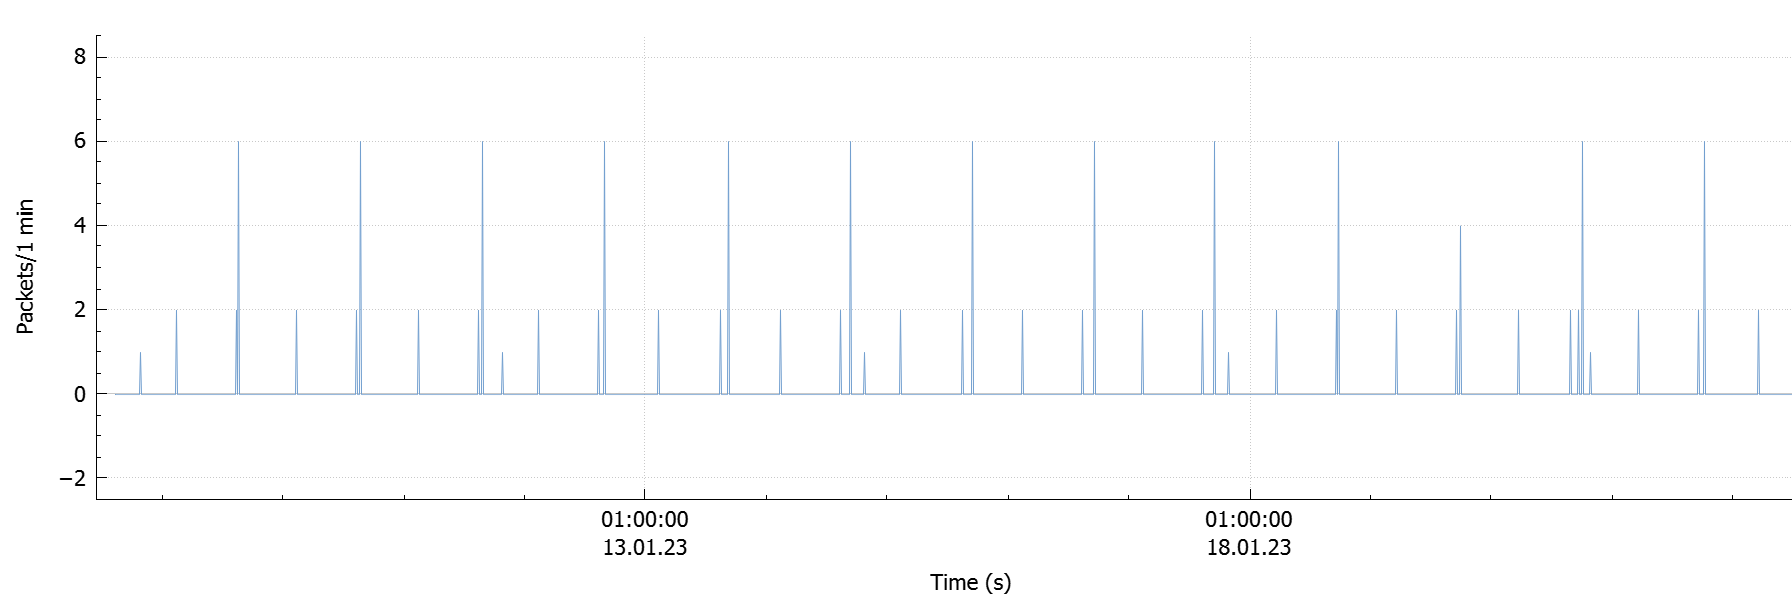
\includegraphics[width=\textwidth]{figures/DNS_irobot_graph.png}
    \caption{Irobot DNS traffic presented in graph}
    \label{fig:dns_irobot_graph}
\end{figure}

The DNS observations identifies that the Irobot Roomba is depending in DNS to be able to access Irobot's cloud services. This protocol is a potentially indication of cloud functionality used or access by the Irobot Roomba and is included in further analysis of events. DNS request for \textit{a.root-servers.net} had to be excluded due to the large amount. All Irobot DNS requests had a packet size larger then 78 bytes as shown in Figure \ref{fig:dns_a-root} and all responses was also larger then the response for \textit{a.root-server.net}. As the DNS response is the most interesting part of the communication it is safe to exclude all DNS packets smaller then 94 bytes without missing any DNS responses towards the Irobot Roomba. 

NTP server-client sessions are identified every 30 minutes generation a large volume of NTP traffic. When observing DNS requests to Irobot's public NTP service \textit{0.irobot.pool.ntp.org} and the NTP traffic it us possible to identify that the Irobot is changing the IP address where the NTP traffic is sent, this is shown in Figure \ref{fig:irobot_ntp_dns}. Since the NTP traffic is continuously it is not related to events triggered, and can be excluded from further analysis by adding the logical expression \textit{!ntp} to the base filter.

\begin{figure}[H]
    \centering
    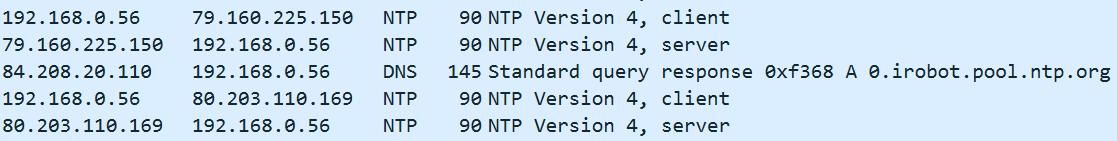
\includegraphics[width=\textwidth]{figures/NTP-irobot.png}
    \caption{Irobot NTP client-server traffic}
    \label{fig:irobot_ntp_dns}
\end{figure}
